\documentclass{article}\usepackage[]{graphicx}\usepackage[]{xcolor}
% maxwidth is the original width if it is less than linewidth
% otherwise use linewidth (to make sure the graphics do not exceed the margin)
\makeatletter
\def\maxwidth{ %
  \ifdim\Gin@nat@width>\linewidth
    \linewidth
  \else
    \Gin@nat@width
  \fi
}
\makeatother

\definecolor{fgcolor}{rgb}{0.345, 0.345, 0.345}
\newcommand{\hlnum}[1]{\textcolor[rgb]{0.686,0.059,0.569}{#1}}%
\newcommand{\hlstr}[1]{\textcolor[rgb]{0.192,0.494,0.8}{#1}}%
\newcommand{\hlcom}[1]{\textcolor[rgb]{0.678,0.584,0.686}{\textit{#1}}}%
\newcommand{\hlopt}[1]{\textcolor[rgb]{0,0,0}{#1}}%
\newcommand{\hlstd}[1]{\textcolor[rgb]{0.345,0.345,0.345}{#1}}%
\newcommand{\hlkwa}[1]{\textcolor[rgb]{0.161,0.373,0.58}{\textbf{#1}}}%
\newcommand{\hlkwb}[1]{\textcolor[rgb]{0.69,0.353,0.396}{#1}}%
\newcommand{\hlkwc}[1]{\textcolor[rgb]{0.333,0.667,0.333}{#1}}%
\newcommand{\hlkwd}[1]{\textcolor[rgb]{0.737,0.353,0.396}{\textbf{#1}}}%
\let\hlipl\hlkwb

\usepackage{framed}
\makeatletter
\newenvironment{kframe}{%
 \def\at@end@of@kframe{}%
 \ifinner\ifhmode%
  \def\at@end@of@kframe{\end{minipage}}%
  \begin{minipage}{\columnwidth}%
 \fi\fi%
 \def\FrameCommand##1{\hskip\@totalleftmargin \hskip-\fboxsep
 \colorbox{shadecolor}{##1}\hskip-\fboxsep
     % There is no \\@totalrightmargin, so:
     \hskip-\linewidth \hskip-\@totalleftmargin \hskip\columnwidth}%
 \MakeFramed {\advance\hsize-\width
   \@totalleftmargin\z@ \linewidth\hsize
   \@setminipage}}%
 {\par\unskip\endMakeFramed%
 \at@end@of@kframe}
\makeatother

\definecolor{shadecolor}{rgb}{.97, .97, .97}
\definecolor{messagecolor}{rgb}{0, 0, 0}
\definecolor{warningcolor}{rgb}{1, 0, 1}
\definecolor{errorcolor}{rgb}{1, 0, 0}
\newenvironment{knitrout}{}{} % an empty environment to be redefined in TeX

\usepackage{alltt}
\usepackage[sc]{mathpazo}
\renewcommand{\sfdefault}{lmss}
\renewcommand{\ttdefault}{lmtt}
\usepackage[T1]{fontenc}
\usepackage{geometry}
\geometry{verbose,tmargin=2.5cm,bmargin=2.5cm,lmargin=2.5cm,rmargin=2.5cm}
\setcounter{secnumdepth}{2}
\setcounter{tocdepth}{2}
\usepackage[unicode=true,pdfusetitle,
 bookmarks=true,bookmarksnumbered=true,bookmarksopen=true,bookmarksopenlevel=2,
 breaklinks=false,pdfborder={0 0 1},backref=false,colorlinks=false]
 {hyperref}
\hypersetup{
 pdfstartview={XYZ null null 1}}

\makeatletter
%%%%%%%%%%%%%%%%%%%%%%%%%%%%%% User specified LaTeX commands.
\renewcommand{\textfraction}{0.05}
\renewcommand{\topfraction}{0.8}
\renewcommand{\bottomfraction}{0.8}
\renewcommand{\floatpagefraction}{0.75}

\makeatother
\IfFileExists{upquote.sty}{\usepackage{upquote}}{}
\begin{document}








The results below are generated from an R script.

\begin{knitrout}
\definecolor{shadecolor}{rgb}{0.969, 0.969, 0.969}\color{fgcolor}\begin{kframe}
\begin{alltt}
\hlkwd{library}\hlstd{(readr)}
\hlkwd{setwd}\hlstd{(}\hlstr{"~/GitHub/dsc520"}\hlstd{)}
\hlstd{scores} \hlkwb{<-} \hlkwd{read_csv}\hlstd{(}\hlstr{"assignments/Week4/scores.csv"}\hlstd{)}
\end{alltt}


{\ttfamily\noindent\itshape\color{messagecolor}{\#\# Rows: 38 Columns: 3\\\#\# -- Column specification ------------------------------------------------------------------\\\#\# Delimiter: "{},"{}\\\#\# chr (1): Section\\\#\# dbl (2): Count, Score\\\#\# \\\#\# i Use `spec()` to retrieve the full column specification for this data.\\\#\# i Specify the column types or set `show\_col\_types = FALSE` to quiet this message.}}\begin{alltt}
\hlcom{# What are the observational units in this study?}
\hlkwd{spec}\hlstd{(scores)}
\end{alltt}
\begin{verbatim}
## cols(
##   Count = col_double(),
##   Score = col_double(),
##   Section = col_character()
## )
\end{verbatim}
\begin{alltt}
\hlkwd{head}\hlstd{(scores)}
\end{alltt}
\begin{verbatim}
## # A tibble: 6 x 3
##   Count Score Section
##   <dbl> <dbl> <chr>  
## 1    10   200 Sports 
## 2    10   205 Sports 
## 3    20   235 Sports 
## 4    10   240 Sports 
## 5    10   250 Sports 
## 6    10   265 Regular
\end{verbatim}
\begin{alltt}
\hlkwd{range}\hlstd{(scores}\hlopt{$}\hlstd{Count)}
\end{alltt}
\begin{verbatim}
## [1] 10 30
\end{verbatim}
\begin{alltt}
  \hlcom{# Count & Score are the observational fields in this study, since the Section is endogenous.}

\hlcom{###}
\hlcom{# Identify the variables mentioned in the narrative paragraph and determine which are categorical and quantitative?}
  \hlcom{# The paragraph identifies the Total Points & Scores as quantitative variables.}
  \hlcom{# We might assume, given the distribution of said variables, that the Score and Count variables represent the aforementioned descriptions.}
  \hlcom{# It's obvious that the categorical variable would the the endogenous Section, given it's datatype and description in the prompt.}

\hlcom{###}
\hlcom{# Create one variable to hold a subset of your data set that contains only the Regular Section and one variable for the Sports Section.}
\hlkwd{library}\hlstd{(dplyr)}
\hlstd{regular} \hlkwb{<-} \hlkwd{filter}\hlstd{(scores, Section} \hlopt{==} \hlstr{'Regular'}\hlstd{)}
\hlstd{sports} \hlkwb{<-}  \hlkwd{filter}\hlstd{(scores, Section} \hlopt{==} \hlstr{'Sports'}\hlstd{)}

\hlcom{###}
\hlcom{# Use the Plot function to plot each Sections scores and the number of students achieving that score.}
\hlcom{# Use additional Plot Arguments to label the graph and give each axis an appropriate label.}

\hlkwd{library}\hlstd{(ggplot2)}
\hlkwd{ggplot}\hlstd{(regular,} \hlkwd{aes}\hlstd{(}\hlkwc{x}\hlstd{=Score,} \hlkwc{y}\hlstd{=Count))} \hlopt{+} \hlkwd{geom_point}\hlstd{(}\hlkwc{color} \hlstd{=} \hlstr{'red'}\hlstd{,} \hlkwc{size} \hlstd{=} \hlnum{2}\hlstd{)} \hlopt{+} \hlkwd{xlab}\hlstd{(}\hlstr{'Scores'}\hlstd{)} \hlopt{+} \hlkwd{ylab}\hlstd{(}\hlstr{'Number of Students'}\hlstd{)} \hlopt{+} \hlkwd{ggtitle}\hlstd{(}\hlstr{'Regular Section Student Scores'}\hlstd{)}
\end{alltt}
\end{kframe}

{\centering 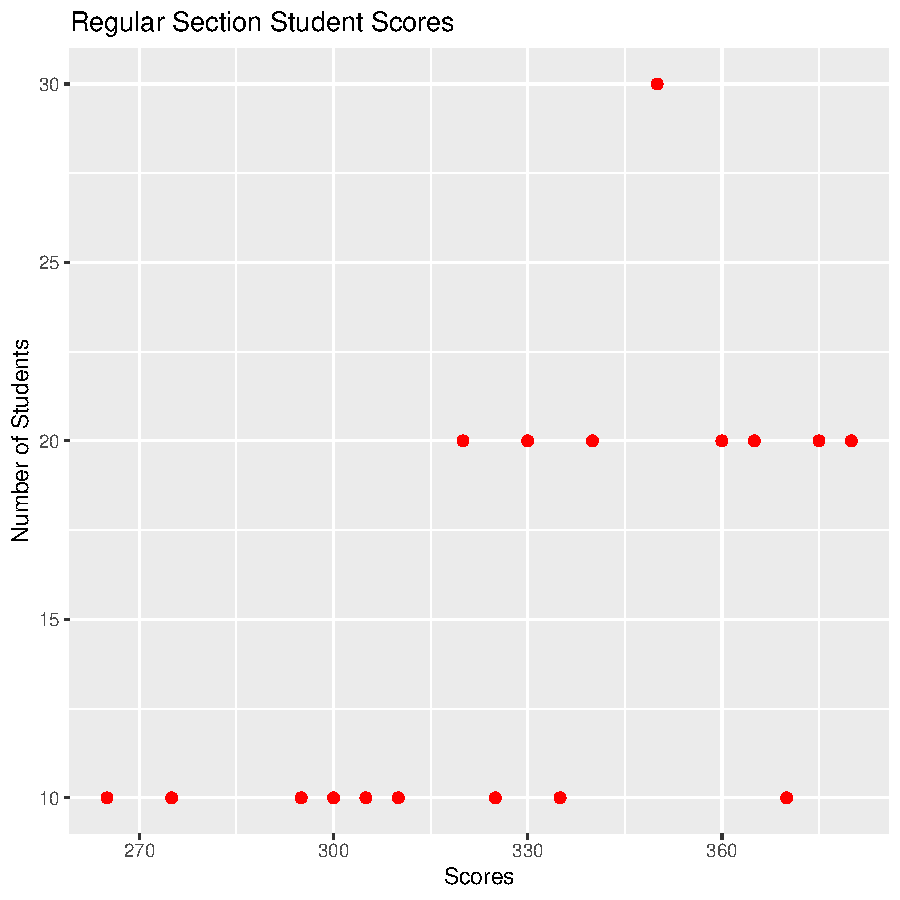
\includegraphics[width=.6\linewidth]{figure/assignment-4-1-SyversonLuke-Rnwauto-report-1} 

}


\begin{kframe}\begin{alltt}
\hlkwd{ggplot}\hlstd{(sports,} \hlkwd{aes}\hlstd{(}\hlkwc{x}\hlstd{=Score,} \hlkwc{y}\hlstd{=Count))} \hlopt{+} \hlkwd{geom_point}\hlstd{(}\hlkwc{color} \hlstd{=} \hlstr{'blue'}\hlstd{,} \hlkwc{size} \hlstd{=} \hlnum{2}\hlstd{)} \hlopt{+} \hlkwd{xlab}\hlstd{(}\hlstr{'Scores'}\hlstd{)} \hlopt{+} \hlkwd{ylab}\hlstd{(}\hlstr{'Number of Students'}\hlstd{)} \hlopt{+} \hlkwd{ggtitle}\hlstd{(}\hlstr{'Sports Section Student Scores'}\hlstd{)}
\end{alltt}
\end{kframe}

{\centering 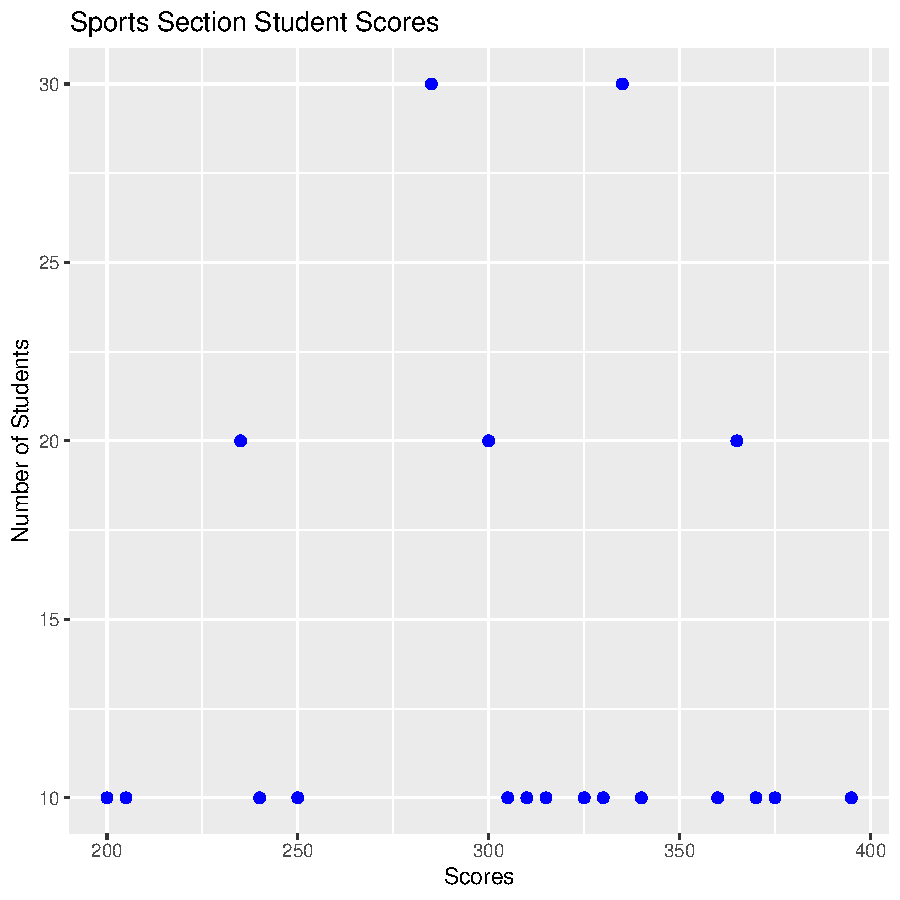
\includegraphics[width=.6\linewidth]{figure/assignment-4-1-SyversonLuke-Rnwauto-report-2} 

}


\begin{kframe}\begin{alltt}
\hlcom{###}
\hlcom{# Once you have produced your Plots answer the following questions:}
\hlcom{# Comparing and contrasting the point distributions between the two section, looking at both tendency and consistency:}
\hlcom{# Can you say that one section tended to score more points than the other? Justify and explain your answer.}

\hlkwd{library}\hlstd{(pastecs)}
\hlkwd{stat.desc}\hlstd{(regular)}
\end{alltt}
\begin{verbatim}
##                    Count        Score Section
## nbr.val       19.0000000   19.0000000      NA
## nbr.null       0.0000000    0.0000000      NA
## nbr.na         0.0000000    0.0000000      NA
## min           10.0000000  265.0000000      NA
## max           30.0000000  380.0000000      NA
## range         20.0000000  115.0000000      NA
## sum          290.0000000 6225.0000000      NA
## median        10.0000000  325.0000000      NA
## mean          15.2631579  327.6315789      NA
## SE.mean        1.4035088    7.6315789      NA
## CI.mean.0.95   2.9486625   16.0333524      NA
## var           37.4269006 1106.5789474      NA
## std.dev        6.1177529   33.2652814      NA
## coef.var       0.4008183    0.1015326      NA
\end{verbatim}
\begin{alltt}
\hlkwd{stat.desc}\hlstd{(sports)}
\end{alltt}
\begin{verbatim}
##                    Count        Score Section
## nbr.val       19.0000000   19.0000000      NA
## nbr.null       0.0000000    0.0000000      NA
## nbr.na         0.0000000    0.0000000      NA
## min           10.0000000  200.0000000      NA
## max           30.0000000  395.0000000      NA
## range         20.0000000  195.0000000      NA
## sum          260.0000000 5840.0000000      NA
## median        10.0000000  315.0000000      NA
## mean          13.6842105  307.3684211      NA
## SE.mean        1.5691705   13.3134085      NA
## CI.mean.0.95   3.2967049   27.9704333      NA
## var           46.7836257 3367.6900585      NA
## std.dev        6.8398557   58.0318021      NA
## coef.var       0.4998356    0.1888021      NA
\end{verbatim}
\begin{alltt}
  \hlcom{# The regular section had higher average and minimum scores, with significantly less variance;}
  \hlcom{# however, the sports section had a higher maximum, and greater variance.}
  \hlcom{# The regular section plots reveal a higher density of scores around the mean than the sports section,}
  \hlcom{# attributing an implied greater probability of higher scores in the regular section.}
  \hlcom{# This leads me to conclude that the regular section tends to score higher.}

\hlcom{###}
\hlcom{# Did every student in one section score more points than every student in the other section? If not, explain what a statistical tendency means in this context.}

  \hlcom{# No, students in each group had varying scores within the same range.}
  \hlcom{# I understand statistical tendency in this context as a unique student's probability of performance,}
  \hlcom{# given their elective participation in the control (regular) or experimental (sports) sections.}

\hlcom{###}
\hlcom{# What could be one additional variable that was not mentioned in the narrative that could be influencing the point distributions between the two sections?}

  \hlcom{# The preexisting performance tendencies of the students could be summarized in their GPAs before beginning the course.}
  \hlcom{# If the GPAs were recorded (assuming them to be accurate historical predictors of class performance),}
  \hlcom{# we might see a bias for higher/lower performing students to enroll in one section over another.}
\end{alltt}
\end{kframe}
\end{knitrout}

The R session information (including the OS info, R version and all
packages used):

\begin{knitrout}
\definecolor{shadecolor}{rgb}{0.969, 0.969, 0.969}\color{fgcolor}\begin{kframe}
\begin{alltt}
\hlkwd{sessionInfo}\hlstd{()}
\end{alltt}
\begin{verbatim}
## R version 4.2.3 (2023-03-15 ucrt)
## Platform: x86_64-w64-mingw32/x64 (64-bit)
## Running under: Windows 10 x64 (build 22000)
## 
## Matrix products: default
## 
## locale:
## [1] LC_COLLATE=English_United States.utf8  LC_CTYPE=English_United States.utf8   
## [3] LC_MONETARY=English_United States.utf8 LC_NUMERIC=C                          
## [5] LC_TIME=English_United States.utf8    
## 
## attached base packages:
## [1] stats     graphics  grDevices utils     datasets  methods   base     
## 
## other attached packages:
## [1] knitr_1.42     pastecs_1.3.21 ggplot2_3.4.1  dplyr_1.1.1    readr_2.1.4   
## 
## loaded via a namespace (and not attached):
##  [1] highr_0.10       pillar_1.9.0     compiler_4.2.3   tools_4.2.3      boot_1.3-28.1   
##  [6] bit_4.0.5        evaluate_0.20    lifecycle_1.0.3  tibble_3.2.1     gtable_0.3.3    
## [11] pkgconfig_2.0.3  rlang_1.1.0      cli_3.6.1        rstudioapi_0.14  parallel_4.2.3  
## [16] xfun_0.38        withr_2.5.0      generics_0.1.3   vctrs_0.6.1      hms_1.1.3       
## [21] bit64_4.0.5      grid_4.2.3       tidyselect_1.2.0 glue_1.6.2       R6_2.5.1        
## [26] fansi_1.0.4      vroom_1.6.1      tzdb_0.3.0       farver_2.1.1     magrittr_2.0.3  
## [31] scales_1.2.1     colorspace_2.1-0 labeling_0.4.2   utf8_1.2.3       munsell_0.5.0   
## [36] crayon_1.5.2
\end{verbatim}
\begin{alltt}
\hlkwd{Sys.time}\hlstd{()}
\end{alltt}
\begin{verbatim}
## [1] "2023-04-09 18:41:25 CDT"
\end{verbatim}
\end{kframe}
\end{knitrout}


\end{document}
